\section{Entropic Swirl Gravity: Verlinde's Holography in a Topological Æther}

The Vortex \AE{}ther Model (VAM) reinterprets gravitation as an emergent phenomenon, not from spacetime curvature, but from structured vorticity and topological information flow in a physically real æther. In this section, we align VAM with the emergent gravity program of Verlinde~\cite{Verlinde2011, Verlinde2016, verlinde2017emergent}, using the tools of swirl dynamics, knot entropy, and vortex-time geometry.

\begin{figure}[h!]
\centering
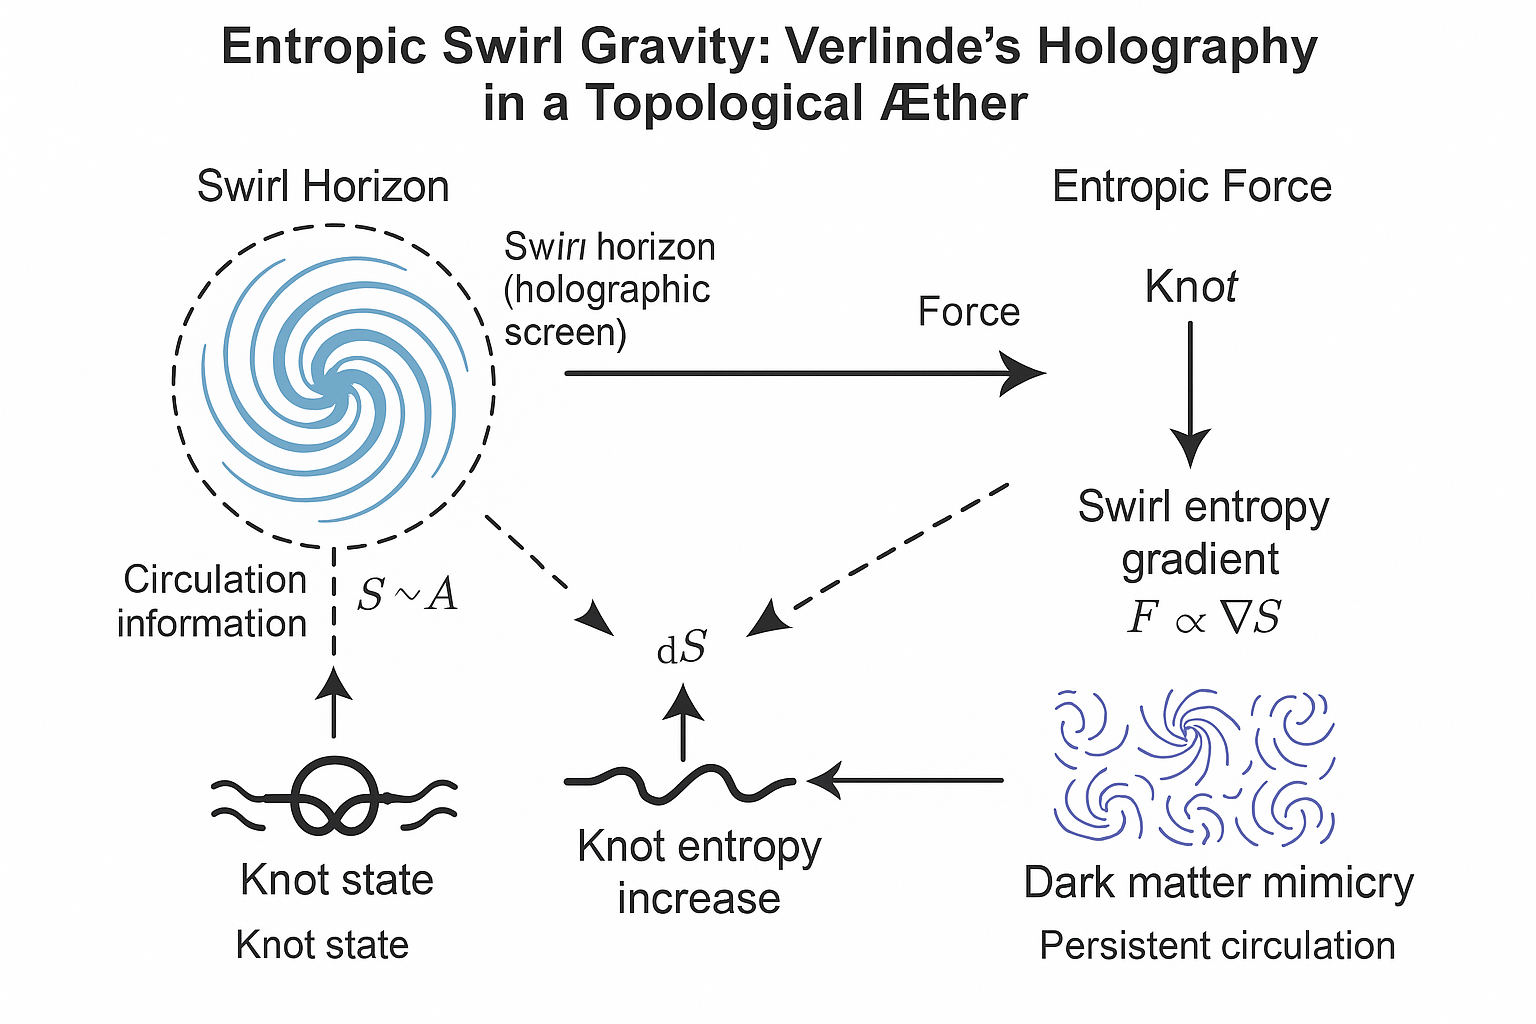
\includegraphics[width=0.65\textwidth]{images/ErikVerlinde}
\caption{%
\textbf{Entropic Swirl Gravity in the VAM framework.}
Swirl horizons in the æther act as holographic information boundaries, encoding the topological microstates of enclosed vortex knots. Entropic gradients in swirl complexity generate emergent forces on probe knots—analogous to Verlinde's entropic gravity. Galactic-scale coherent helicity fields resist entropy diffusion and manifest as dark matter–like inertial structures.
}
\end{figure}

\subsection*{Swirl Entropy and Vortex Microstates}

In Verlinde’s view, gravity arises from gradients in entropy associated with hidden microscopic degrees of freedom. VAM realizes this concretely: the microstates are \emph{topological configurations} of vortex knots—characterized by twist \( T \), chirality \( C \), linking \( Lk \), and knot class \( K \). The local swirl entropy is then:

\begin{equation}
S_{\text{swirl}}(x) = k_B \log \Omega_{\text{topo}}(x),
\end{equation}

where \( \Omega_{\text{topo}} \) is the number of accessible vortex states at position \( x \). A test vortex moving into regions of higher \( \Omega \) experiences an entropic force:

\begin{equation}
F_i = T_{\text{æ}} \, \partial_i S_{\text{swirl}},
\end{equation}

where \( T_{\text{æ}} \) is the effective \ae{}theric temperature, interpreted not thermally but as the rate of topological transitions per unit vortex time \( T_v \).

\subsection*{Holography via Swirl Surfaces}

Verlinde’s holographic screens store bulk information on surface boundaries. In VAM, the natural analog is a \textbf{swirl envelope}: a compact 2D surface enclosing vorticity flux or knotted cores. The entropy associated with this surface obeys:

\begin{equation}
S_{\text{holo}} \propto A_{\text{swirl}},
\end{equation}

where \( A_{\text{swirl}} \) is the integrated helicity flux density crossing the surface. Temporal flow rate within the enclosed region is regulated by swirl clock decoherence \( S(t) \), thus forming a time-holographic correspondence.

\subsection*{Swirl Complexity as Gravitational Source}

In VAM, gravitational attraction arises from gradients in swirl density and knot microstructure. These induce:

\begin{itemize}
    \item \textbf{Time dilation} via reduced helicity flow: \( d\tau \propto \vec{v} \cdot \vec{\omega} \),
    \item \textbf{Entropic attraction} from information imbalance across swirl boundaries,
    \item \textbf{Swirl inertia} from locked phase \( S(t) \) between vortex bundles.
\end{itemize}

This recasts Verlinde’s gravity as a byproduct of circulation dynamics and coherent vortex alignment in the æther manifold \( \mathcal{N} \).

\subsection*{Dark Matter as Ætheric Memory Field}

Verlinde suggests that dark matter effects emerge from residual information fields. In VAM, this is naturally modeled as \emph{long-lived helicity condensates}:

\begin{itemize}
    \item Swirl fields resist dissipation due to topological conservation,
    \item Large-scale swirl coherence stores memory of galactic rotation history,
    \item Local accelerations \( a < a_0 \) fall below the decoherence threshold of knotted domains.
\end{itemize}

This provides a purely fluid-dynamic, time-oriented account of galactic rotation curves—without invoking particle dark matter.

\subsection*{Temporal Ontology Perspective}

Time in VAM is not fundamental, but emergent from vortex topology:

\begin{equation}
d\tau = \lambda (\vec{v} \cdot \vec{\omega}) \, dt,
\end{equation}

where \( d\tau \) is Chronos-Time (observer proper time), \( \vec{v} \cdot \vec{\omega} \) is local helicity density (swirl clock rate), and \( \lambda \sim r_c^2 / C_e^2 \) sets dimensional scaling. This ties together:

\[
\textbf{Swirl} \leftrightarrow \textbf{Temporal Evolution}, \quad
\textbf{Helicity} \leftrightarrow \textbf{Entropy Flux}, \quad
\textbf{Swirl Horizon} \leftrightarrow \textbf{Causal Boundary}.
\]

Thus, VAM reformulates Verlinde's geometric entropy in a mechanically precise temporal framework via \( T_v \), \( S(t) \), and knotted phase decoherence.

\subsection*{Conclusion}

The emergent gravity framework proposed by Verlinde finds a concrete realization in the Vortex \AE{}ther Model. By identifying gravitational forces with swirl-entropy gradients, and time with helicity accumulation, VAM offers:

\begin{itemize}
    \item A physically explicit æther-based holography,
    \item A derivation of gravity from topological dynamics,
    \item A resolution of dark matter via non-dissipative helicity memory,
    \item And a unified clockwork of time, mass, and inertia from vortex ontology.
\end{itemize}

This bridges fluid-topological mechanics with emergent information theory—anchoring entropy, force, and time in the swirl structure of the physical æther.
